\documentclass[journal]{IEEEtran}

\usepackage{cite}
\usepackage{amsmath}
\interdisplaylinepenalty=2500
\usepackage{algorithm}
\usepackage[noend]{algpseudocode}
\usepackage{array}
\usepackage{graphicx}
\usepackage{float}

% correct bad hyphenation here
\hyphenation{op-tical net-works semi-conduc-tor}


\begin{document}
\title{Camera calibration using OpenCV}

\author{Wilbert~Pumacay,~\textit{Catholic University San Pablo},~wilbert.pumacay@ucsp.edu.pe\\
        Gerson~Vizcarra,~\textit{Catholic University San Pablo},~gerson.vizcarra@ucsp.edu.pe}

% make the title area
\maketitle

\begin{abstract}
Camera calibration is an important step in several applications, like augmented reality. To do calibration properly using current calibration methods we need to get features we can related in both 2D camera space and 3D world space to estimate the camera parameters that give this mapping. In this context, the use of grid patterns help by giving us the features we need, being the components in the pattern which we must detect in every frame in video.
\\
\\
In this paper we use Zhang \cite{CameraCalibration1} camera calibration technique implemented by OpenCV, and compare results using feature extraction of chessboard corners, symmetric/asymmetric circle grids, and concentric circle grid patterns, the first two, using funnctions implemented in OpenCV and the third one using our own algorithm by implementing a pipeline that gets these features by combining various techniques from classical image processing.
\end{abstract}

\begin{IEEEkeywords}
Camera calibration, calibration pattern, circle grid, image processing.
\end{IEEEkeywords}


\section{Introduction}

\IEEEPARstart{T}{he} camera calibration problem consists of finding 11 parameters that describe the mapping between 2D camera space and 3D world space. Six parameters, called extrinsic, come from an homogeneous transform, giving 6 parameters ( rotation and translation around the axes ). The other 5 parameters, called intrinsic, define some internal properties of the camera. This can be expressed in the following transformation equation:

\begin{equation}
  \begin{bmatrix}
    \mu \\
    \nu \\
      1 
  \end{bmatrix} = 
  \begin{bmatrix}
    \alpha & \gamma & \mu_{0} \\
       0   & \beta  & \nu_{0} \\
       0   &    0   &    1
  \end{bmatrix} 
  \begin{bmatrix}
    r_{x_{1}} & r_{y_{1}} & r_{z_{1}} & t_{x}\\
    r_{x_{2}} & r_{y_{2}} & r_{z_{2}} & t_{y}\\
    r_{x_{3}} & r_{y_{3}} & r_{z_{3}} & t_{z}
  \end{bmatrix} 
  \begin{bmatrix}
    x \\
    y \\
    z \\
    1
  \end{bmatrix}
%
\end{equation}

In this equation we can detail each of the variables: $x,y,z$ are original coordinates of an object, $r_{ij}$ and $t_{ij}$ means the rotation and translation values respectively in the model matrix, $\alpha$ and $\beta$ represents the focal length in x and y axis respectively, $\mu_0$ and $\nu_0$ are the coordinates x and y at the optical center.
\\
\\
To find these parameters, camera calibration methods make use of correspondences between 2D and 3D spaces in order to fit the parameters that best describe this mapping. We achieve this by minimizing the following function:

\begin{equation}
  \sum^{m}_{i} \sum^{n}_{j} \Vert TP^{ij}_{3D} - P^{ij}_{2D} \Vert^{2}
\end{equation}

Where we are trying to minimize the difference between the expected projection and the actual projection over some set of features. The key idea is that supplying sufficient features that have a correct mapping, we can get the 11 parameters needed that minimize this function. So, a key part is the detection of these features.
\\
\\
In equation $2$ we are looping through a set of features $n$ that are found in each frame of a video of $m$ frames, so, we basically need to detect some feature points in each frame of video, which is what we focus in this paper.

\section{About the method}
To compare results of feature extraction, we implemented the following pipeline.

\begin{figure}[H]
\centering
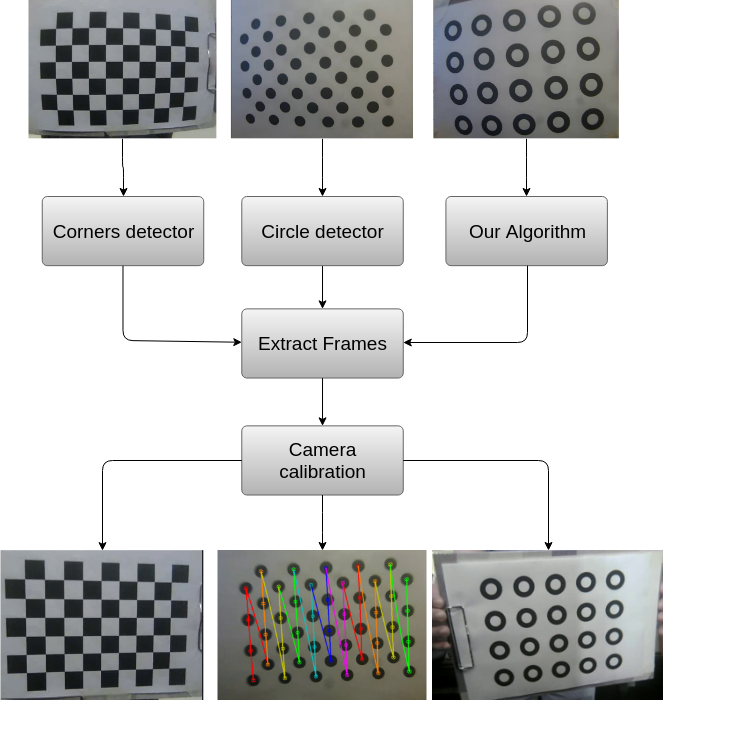
\includegraphics[width=2.5in]{_img/img_report3_pipeline.png}
\caption{Comparison pipeline.}
\end{figure}

\subsection{ Pattern detection }
We used three principal patterns to calibrate the camera with OpenCV calibration: Chessboard pattern, Circle symmetric/asymmetric pattern and circle concentric pattern. In the first two patterns we applied OpenCV implemented functions, in chessboard pattern we have to recognize corners and save their position, in circle pattern we have to detect circles and save the position of their centers.

\subsection{Circle concentric pattern detection}
The pipeline of our pattern detection and tracking algorithm works as follows:

\begin{figure}[H]
\centering
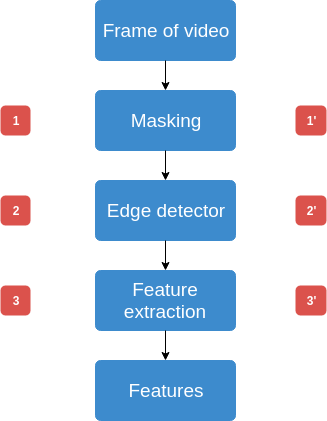
\includegraphics[width=2.5in]{_img/algorithm_overview.png}
\caption{Pipeline of previous work.}
\end{figure}

\subsubsection{ Masking }
This step is in charge of isolating the pattern by using threhsolding operations.
\\
\\
The approach consists on creating a mask from the grayscale transformed image applying \textbf{Adaptive Thresholding algorithm}, this algorithm relies on Integral Image technique especified in \cite{IntegralImageThresholding}.
\begin{algorithm}
\caption{Masking}
\label{alg:mask2}
\begin{algorithmic}[1]
\State $\textit{Set up thresholding parameters}$
\State $mask   = \textit{rgb2gray}( inputImage )$
\State $mask   = \textit{AdaptiveThreshold}(mask, blockSize)$\\
\Return $masked$
\end{algorithmic}
\end{algorithm}
%%%%%%%%%%%%%%%%%%%%%%%%%%%%%%%%%%%%%%%%%%%%%%%%%%%%%%%
\begin{figure}[H]
\centering
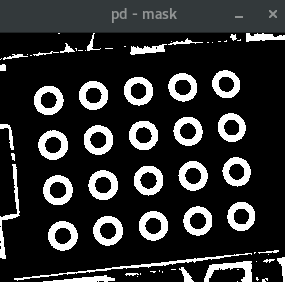
\includegraphics[width=2.5in]{_img/img_report2_mask.png}
\caption{Image mask applied to ROI.}
\end{figure}

\subsubsection{Edge detection}
In this stage of the pipeline we extract edges from the result of the previous stage. In order to do this, we applied \textbf{Scharr operators} on \textit{x} and \textit{y} axis (as described in algorithm 2); Scharr is the result from Sobel algorithm minimizing weighted mean squared angular error in Fourier domain.
%% TODO: Gerson
\begin{algorithm}
\caption{Edge detection}
\begin{algorithmic}[1]
\State $axis_x   = \textit{Scharr}(masked, 1, 0)$
\State $axis_x   = \textit{Abs}(axis_x)$
\State $axis_y   = \textit{Scharr}(masked, 0, 1)$
\State $axis_y   = \textit{Abs}(axis_y)$
\State $edgesImage   = \textit{Add}(axis_x, axis_y)$ \\
\Return $edgesImage$
\end{algorithmic}
\end{algorithm}

\begin{figure}[H]
\centering
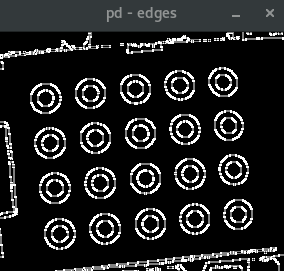
\includegraphics[width=2.5in]{_img/img_report2_edges.png}
\caption{Edge detection to mask.}
\end{figure}

\subsubsection{Feature extraction}
The last stage consist of extracting the features needed for the calibration from the edges detected in the previous stage. We used OpenCV's \textbf{SimpleBlobDetector} that applies an extra thresholding on the image, applies the \textbf{findContours} algorithm to calculate the blob centers, groups centers of several images by their coordinates in blobs and finally, estimates the final centers of the blobs. For detecting only pattern blobs, we had to apply similar heuristics to above (color blobs, area, aspect ratio, and convexity of points).

\begin{figure}[H]
\centering
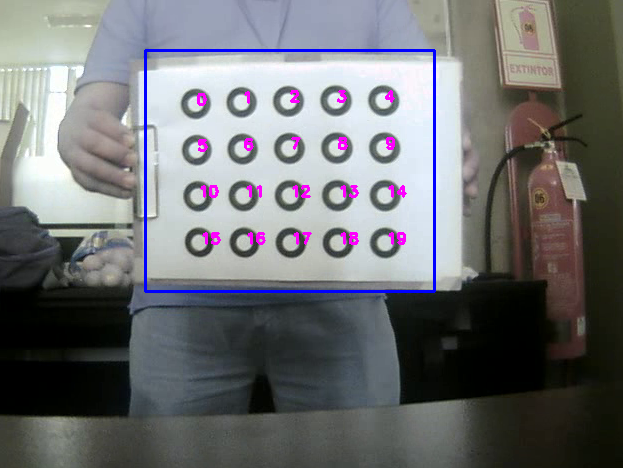
\includegraphics[width=2.5in]{_img/img_report2_feature_detection.png}
\caption{Result after feature detection.}
\end{figure}

\subsection{Pattern Matching and Ordering}
Once we have the features extracted, we have to order them for them to be used in the calibration algorithm. To achieve this, we made a simple algorithm that matches the best candidate grid to the current features, and correct by the orientation in order to choose a correct ordering.
\\
\\
We first create a bounding box of the current possible corners. Then, we take the outer most corners as the corners of the pattern. With this information, we can compute a candidate grid that represents the positions where the candidate points should be, as seen in figure 7.

\begin{figure}[H]
\centering
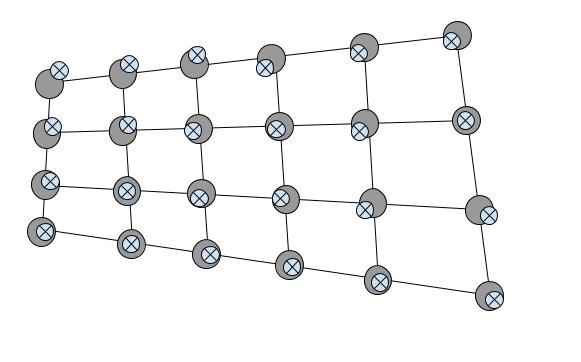
\includegraphics[width=2.5in]{_img/img_report3_pattern_matching.jpg}
\caption{Grid pattern matching.}
\end{figure}

We check for each combination of outer most corners, which ordering gives the best fit. This will give us a correct ordering of the outer most corners of the pattern.
\\
\\
Lastly, we check that the orientation of the board is in some range, as shown in figure 8, which will complete the corner ordering, as shown in figure 9.
\\
\\
\begin{figure}[H]
\centering
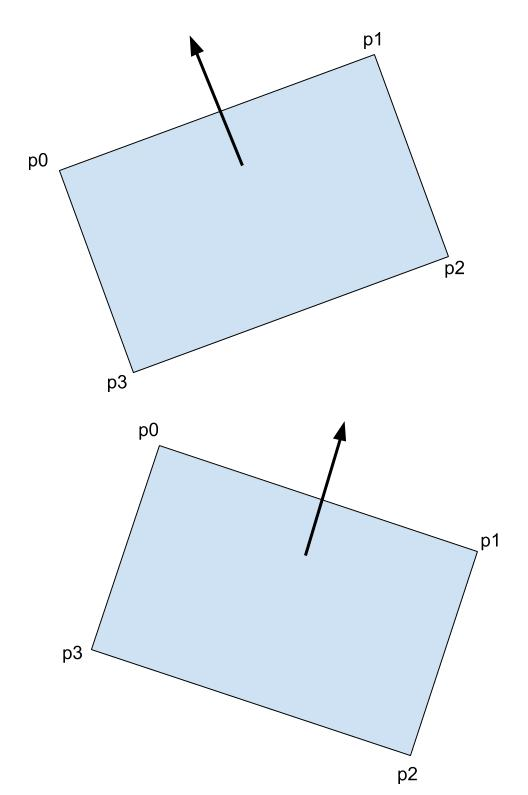
\includegraphics[width=2.5in]{_img/img_pattern_orientation_checking.jpg}
\caption{Pattern orientation check.}
\end{figure}

\begin{figure}[H]
\centering
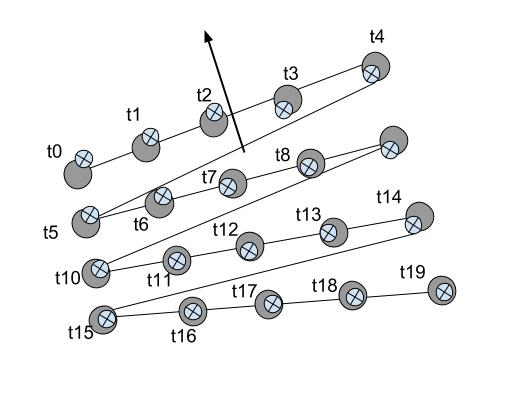
\includegraphics[width=2.5in]{_img/img_report3_pattern_order_check.jpg}
\caption{Pattern final ordering after matching.}
\end{figure}

\section{Results}
We calibrated two cameras using as feature detection the three detection algorithms described earlier ( OpenCV's chessboard and circle finder and our algorithm )

For each calibration, we took a fixed batch of 30 correctly processed images. The results are the following :
\\
\\
\begin{table}[H]
\begin{tabular}{ |p{2cm}||p{2cm}|p{2cm}|p{2cm}|  }
 \hline
 Parameter & Chessboard & Asymmetric & Rings \\
 \hline
 fx        & 609.6& 609.5& 627.0\\
 fy        & 609.4& 612.6& 631.8\\
 vx        & 326.9& 351.5& 342.7\\
 vy 	   & 223.8& 227.2& 231.2\\
 RMS error & 0.74 & 0.22 & 0.19\\
 \hline
\end{tabular}
\\
\caption{MS Life Cam calibration}
\end{table}

\begin{table}[H]
\begin{tabular}{ |p{2cm}||p{2cm}|p{2cm}|p{2cm}|  }
 \hline
 Parameter & Chessboard & Asymmetric & Rings \\
 \hline
 fx        & 876.2& 933.2& 829.5\\
 fy        & 876.6& 935.4& 834.8\\
 vx        & 325.0& 342.3& 320.0\\
 vy 	   & 251.4& 220.7& 243.5\\
 RMS error & 0.313& 0.184& 0.187\\
 \hline
\end{tabular}
\\
\caption{PS3 Eye Cam calibration}
\end{table}

\section{Conclusions and Future improvements}
We see by the results that our algorithm is close enough compared to OpenCV's pattern detectors. We got close to the camera matrix parameters obtained by the other detector algorithms.

Also, the matching and ordering algorithm allows us to get the right ordering, allowing us to pick the right calibration frames to be used for the calibration process.

This process is still quite cumbersome because we have to pick each frame that we want to use. We plan on making this process automatic, by keeping frames at some fixed rate and checking that we pick the right combination of frames from a big batch that give us a good overall distribution over the whole field of view. We have made some tools to help us with this task, as shown in Fig. 9.

\begin{figure}[H]
\centering
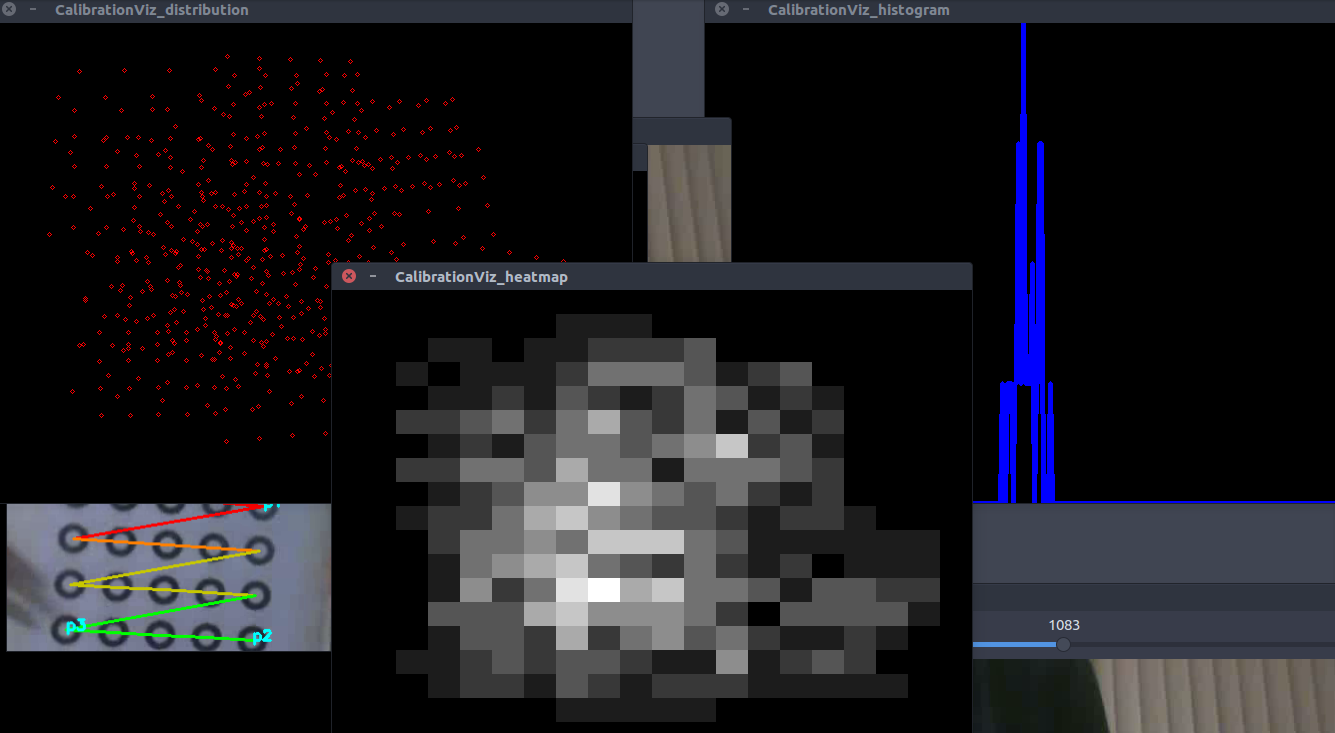
\includegraphics[width=2.5in]{_img/tools.png}
\caption{Pattern final ordering after matching.}
\end{figure}

We have a heat-map that give us a distribution visualizer, as well as a histogram to be sure we are picking the patterns at some range of orientations. 

\IEEEtriggeratref{8}

% references section
\begin{thebibliography}{1}

\bibitem{OpenCV}
  Bradski, G. \\
  \textit{OpenCV library.} - 2000
\\
\bibitem{CameraCalibration1}
  Zhengyou Zhang \\
  \textit{A Flexible New Technique for Camera Calibration.} - 2000
\\
\bibitem{IntegralImageThresholding}
  Derek Bradley, Gerhard Roth \\
  \textit{Adaptive Thresholding Using the Integral Image.} - 2011

\end{thebibliography}


\end{document}

